%-------------------------------------------------------------------------------
%
% TUM Dissertation Template
%
% For usage instructions see README.md
%
% Authors:
%   Andre Richter, andre.richter@tum.de
%   Michael Vonbun, michael.vonbun@tum.de
%   Christian Herber, christian.herber@tum.de
%   Stefan Wallentowitz, stefan.wallentowitz@tum.de
%
%-------------------------------------------------------------------------------
\documentclass[%
  % layouttitlepage,            % layout help rules (to see if you need
  %                             % some extra vspace in your title etc.)
  headings = standardclasses, % serif fonts for headings
  % headings = big,             % If you use serif fonts for headings (above option
  %                             % uncommmented), uncomment this one to get smaller
  %                             % headings
  % sansseriftitlepage,         % sans serif title page
]{tumDiss}
\usepackage[utf8]{inputenc}



%-------------------------------------------------------------------------------
% Binding correction for the title page.
% WARNING: ONLY NEEDED FOR THE PRINT VERSION!
%
% After printing and binding, the left part of the titlepage may lose
% significant space, for example due to overlap from glue binding.
% You can increase the left margin of the title page with this option.
% This value of 8mm was measured for glue binding a thesis that was printed by
% the TUM Fachschaft EI and ~140 pages.
%-------------------------------------------------------------------------------
% \titlepagebindingcor{8mm}

%-------------------------------------------------------------------------------
% Binding correction for everything else.
% Does not affect titlePageBindingCor!
%
% WARNING: THIS OPTION CAN SHAKE UP YOUR CURRENT LAYOUT.
% If you want to use it, it is best to work with it from the very start. Adding
% it when finishing your dissertation might get you into trouble.
%
% Search http://texdoc.net/texmf-dist/doc/latex/koma-script/scrguien.pdf for
% "BCOR" for further reading.
%-------------------------------------------------------------------------------
% \KOMAoptions{BCOR=3mm}



%-------------------------------------------------------------------------------
% Faculty
%-------------------------------------------------------------------------------
\faculty{Ingenieurfakultät Bau Geo Umwelt}

%-------------------------------------------------------------------------------
% Degree
%-------------------------------------------------------------------------------
\degree{Doktor-Ingenieurs (Dr.-Ing.)}

%-------------------------------------------------------------------------------
% Title
%
% IMPORTANT:
%
% You must add manual line breaks here. If you don't, you'll get uneven spacing
% between the lines.
% YOU ALSO NEED THE BREAK AT THE LAST LINE.
%-------------------------------------------------------------------------------
\title{%
  Fusion of Images Acquired From Airplanes and Unmanned Aerial Vehicles (UAVs) in Scene Awareness Applications\\
}
% \subtitle{That is extended by using an additional subtitle}

%-------------------------------------------------------------------------------
% People
%-------------------------------------------------------------------------------
\author{Xiangyu Zhuo, M.Sc.}
\vorsitz{X}
\erstpruef{Univ.-Prof. Dr.-Ing. habil. Richard H. G. Bamler}

% Use this one for a TUM professor
% \zweitpruef{}

% Or this one for an external professor
\zweitpruef[Technische Universität Graz, Österreich]{Ass.Prof. Dipl.-Ing. Dr. techn. Friedrich Fraundorfer}

% Optionally, add a third examiner
\drittpruef[Universität Osnabrück]{Prof. Dr.-Ing. Peter Reinartz}

%-------------------------------------------------------------------------------
% Hand in date
%
% This is the date of your personal hand-in at the TUM doctoral office.
%-------------------------------------------------------------------------------
\date{01.01.2016}

%-------------------------------------------------------------------------------
% Accepted date
%
% You can set this after your thesis was accepted. For handing in,
% it is not needed (at least for the Electrical Engineering faculty).
%-------------------------------------------------------------------------------
\dateaccepted{10.05.2016}



%-------------------------------------------------------------------------------
% Change language, e.g. to german
%-------------------------------------------------------------------------------
% \usepackage[ngerman]{babel}

%-------------------------------------------------------------------------------
% Compatibility issues
%-------------------------------------------------------------------------------
% If you need pstricks, load it here before everything else.
% Otherwise, tikz patterns won't work
%\usepackage{pstricks}

%-------------------------------------------------------------------------------
% Suggested standard packets are included here
%-------------------------------------------------------------------------------
% Loading scrhack fixes:
%   (1) KOMA-Script incompatible macros used in listings package.
%   (2) Inconsistent anchors in hyperref.

\usepackage{scrhack}

% glossary functionality
\usepackage[
  toc,
  acronym,
  style = long
]{glossaries}
\makeglossaries

% figure inclusion
% \usepackage[
%   caption = false,
%   font    = footnotesize
% ]{subfig}
\usepackage{graphicx}
\graphicspath{{./Figures/}}
\usepackage{pgfplots}
\usepackage{pgfplotstable}
\tikzset{>=stealth}
\usetikzlibrary{patterns}
\usetikzlibrary{pgfplots.statistics}

% code block insertion
\usepackage{moreverb}
\usepackage{listings}

% math and equations
\usepackage{amsmath}
\usepackage{amssymb}
\usepackage{amsfonts}
\usepackage{upgreek}

% enumeration
\usepackage{enumerate}

% hyperlinks
\usepackage{url}
\usepackage[
  hidelinks,
  bookmarksnumbered
]{hyperref}


% If hyperref is used, references to tables and figures link to their captions
% and not the actual tables or figures. This is especially unwanted for figures,
% because their captions are below the figure so that clicking on a link just
% shows the captions and the figure is invisible.
%
% Using the caption package fixes this behaviour.
\usepackage{caption}

% Source code with highlighting
\usepackage{listings}
\lstset{
  basicstyle       = \footnotesize,
  captionpos       = b,
  tabsize          = 4,
  commentstyle     = \color{TUMGreen},
  keywordstyle     = \color{TUMBlue},
  stringstyle      = \color{TUMOrange},
  otherkeywords    = {
    uint64_t,
    uint32_t,
    uint16_t,
    uint8_t,
    u64,
    u32,
    u16,
    u8,
    inline
  },
  numbers          = left,
  xleftmargin      = 7ex,
  aboveskip        = 4ex,
  abovecaptionskip = 2ex,
}

% Support for siunitx
\usepackage{siunitx}
\sisetup{
  exponent-product = \cdot,
  output-product   = \cdot,
  per-mode         = symbol-or-fraction,
  quotient-mode    = fraction,
  binary-units     = true
}

% No widows and orphans
\usepackage[all]{nowidow}

% dummy text
\usepackage{lipsum}

%-------------------------------------------------------------------------------
% Include custom packages here
%-------------------------------------------------------------------------------

\usepackage[official]{eurosym}
\usepackage{booktabs}
\usepackage{subcaption}
\usepackage{float}
\usepackage{pgfplots}
\usepackage{tikz}
\usetikzlibrary{spy,calc}
\usepackage[export]{adjustbox}
%-------------------------------------------------------------------------------
% TUM CI colors for PGF
%-------------------------------------------------------------------------------
\definecolor{grey60} {RGB} {102, 102, 102} % 60% grey

\pgfplotscreateplotcyclelist{tum}{
  {color = TUMBlack,        mark = o,                     mark size = 3.8},
  {color = TUMBlue,         mark = star,                  mark size = 3.8},
  {color = TUMBlueDarker,   mark = square,                mark size = 3.8},
  {color = TUMBlueLighter,  mark = triangle,              mark size = 3.8},
  {color = TUMBlueDarkest,  mark = diamond,               mark size = 3.8},
  {color = TUMBlueLightest, mark = |,                     mark size = 3.8},
  %%
  {color = TUMBlack,        mark = *,                     mark size = 3.8},
  {color = TUMBlue,         mark = 10-pointed star,       mark size = 3.8},
  {color = TUMBlueDarker,   mark = square*,               mark size = 3.8},
  {color = TUMBlueLighter,  mark = triangle*,             mark size = 3.8},
  {color = TUMBlueDarkest,  mark = diamond*,              mark size = 3.8},
  {color = TUMBlueLightest, mark = Mercedes star flipped, mark size = 3.8}
}

\pgfplotsset{/pgfplots/bar cycle list/.style={/pgfplots/cycle list={
      {black, mark = none, fill = TUMBlue},
      {black, mark = none, fill = TUMBlueLightest},
      {black, mark = none, pattern = north east lines, pattern color = TUMBlue},
      {black, mark = none, pattern = north west lines, pattern color = TUMBlue},
      {black, mark = none, pattern = north east lines, pattern color = TUMOrange},
      {black, mark = none, pattern = north west lines, pattern color = TUMOrange},
      {black, mark = none, pattern = horizontal lines, pattern color = TUMOrange},
      {black, mark = none, pattern = crosshatch,       pattern color = TUMOrange}
    }
  }
}

%-------------------------------------------------------------------------------
% Default values for pgfplots
%-------------------------------------------------------------------------------
\newcommand{\figureHeight}{0.5625} %% 16:9
\pgfplotsset{
  compat           = 1.13,
  grid             = major,
  enlarge x limits = 0,
  cycle list name  = tum,
  major grid style = {dotted},
  minor grid style = {dotted},
  legend style     = {
    at     = {(0.98,0.96)},
    anchor = north east,
  },
  width            = \hsize * 0.9,
  height           = \hsize * 0.9 * \figureHeight,
}

%-------------------------------------------------------------------------------
% Correct bad hyphenation here
%-------------------------------------------------------------------------------
\hyphenation{op-tical net-works semi-conduc-tor}

%-------------------------------------------------------------------------------
% Acronyms (will be sorted alphabetically)
%-------------------------------------------------------------------------------
\newacronym{cpu}{CPU}{Central Processing Unit}
\glsadd{cpu}

\newacronym{pci}{PCI}{Peripheral Component Interconnect}
\glsadd{pci}

\newacronym{pcie}{PCIe}{Peripheral Component Interconnect Express}
\glsadd{pcie}

\newacronym{mmu}{MMU}{Memory Management Unit}
\glsadd{mmu}


%---------------spy effect----------------------
\newif\ifblackandwhitecycle
\gdef\patternnumber{0}

\pgfkeys{/tikz/.cd,
    zoombox paths/.style={
        draw=orange,
        very thick
    },
    black and white/.is choice,
    black and white/.default=static,
    black and white/static/.style={ 
        draw=white,   
        zoombox paths/.append style={
            draw=white,
            postaction={
                draw=black,
                loosely dashed
            }
        }
    },
    black and white/static/.code={
        \gdef\patternnumber{1}
    },
    black and white/cycle/.code={
        \blackandwhitecycletrue
        \gdef\patternnumber{1}
    },
    black and white pattern/.is choice,
    black and white pattern/0/.style={},
    black and white pattern/1/.style={    
            draw=white,
            postaction={
                draw=black,
                dash pattern=on 2pt off 2pt
            }
    },
    black and white pattern/2/.style={    
            draw=white,
            postaction={
                draw=black,
                dash pattern=on 4pt off 4pt
            }
    },
    black and white pattern/3/.style={    
            draw=white,
            postaction={
                draw=black,
                dash pattern=on 4pt off 4pt on 1pt off 4pt
            }
    },
    black and white pattern/4/.style={    
            draw=white,
            postaction={
                draw=black,
                dash pattern=on 4pt off 2pt on 2 pt off 2pt on 2 pt off 2pt
            }
    },
    zoomboxarray inner gap/.initial=5pt,
    zoomboxarray columns/.initial=2,
    zoomboxarray rows/.initial=2,
    subfigurename/.initial={},
    figurename/.initial={zoombox},
    zoomboxarray/.style={
        execute at begin picture={
            \begin{scope}[
                spy using outlines={%
                    zoombox paths,
                    width=\imagewidth / \pgfkeysvalueof{/tikz/zoomboxarray columns} - (\pgfkeysvalueof{/tikz/zoomboxarray columns} - 1) / \pgfkeysvalueof{/tikz/zoomboxarray columns} * \pgfkeysvalueof{/tikz/zoomboxarray inner gap} -\pgflinewidth,
                    height=\imageheight / \pgfkeysvalueof{/tikz/zoomboxarray rows} - (\pgfkeysvalueof{/tikz/zoomboxarray rows} - 1) / \pgfkeysvalueof{/tikz/zoomboxarray rows} * \pgfkeysvalueof{/tikz/zoomboxarray inner gap}-\pgflinewidth,
                    magnification=3,
                    every spy on node/.style={
                        zoombox paths
                    },
                    every spy in node/.style={
                        zoombox paths
                    }
                }
            ]
        },
        execute at end picture={
            \end{scope}
             \node at (image.north) [anchor=north,inner sep=0pt] {\subcaptionbox{\label{\pgfkeysvalueof{/tikz/figurename}-image}}{\phantomimage}};
              \node at (zoomboxes container.north) [anchor=north,inner sep=0pt] {\subcaptionbox{\label{\pgfkeysvalueof{/tikz/figurename}-zoom}}{\phantomimage}};
     \gdef\patternnumber{0}
        },
        spymargin/.initial=0.5em,
        zoomboxes xshift/.initial=1,
        zoomboxes right/.code=\pgfkeys{/tikz/zoomboxes xshift=1},
        zoomboxes left/.code=\pgfkeys{/tikz/zoomboxes xshift=-1},
        zoomboxes yshift/.initial=0,
        zoomboxes above/.code={
            \pgfkeys{/tikz/zoomboxes yshift=1},
            \pgfkeys{/tikz/zoomboxes xshift=0}
        },
        zoomboxes below/.code={
            \pgfkeys{/tikz/zoomboxes yshift=-1},
            \pgfkeys{/tikz/zoomboxes xshift=0}
        },
        caption margin/.initial=4ex,
    },
    adjust caption spacing/.code={},
    image container/.style={
        inner sep=0pt,
        at=(image.north),
        anchor=north,
        adjust caption spacing
    },
    zoomboxes container/.style={
        inner sep=0pt,
        at=(image.north),
        anchor=north,
        name=zoomboxes container,
        xshift=\pgfkeysvalueof{/tikz/zoomboxes xshift}*(\imagewidth+\pgfkeysvalueof{/tikz/spymargin}),
        yshift=\pgfkeysvalueof{/tikz/zoomboxes yshift}*(\imageheight+\pgfkeysvalueof{/tikz/spymargin}+\pgfkeysvalueof{/tikz/caption margin}),
        adjust caption spacing
    },
    calculate dimensions/.code={
        \pgfpointdiff{\pgfpointanchor{image}{south west} }{\pgfpointanchor{image}{north east} }
        \pgfgetlastxy{\imagewidth}{\imageheight}
        \global\let\imagewidth=\imagewidth
        \global\let\imageheight=\imageheight
        \gdef\columncount{1}
        \gdef\rowcount{1}
        \gdef\zoomboxcount{1}
    },
    image node/.style={
        inner sep=0pt,
        name=image,
        anchor=south west,
        append after command={
            [calculate dimensions]
            node [image container,subfigurename=\pgfkeysvalueof{/tikz/figurename}-image] {\phantomimage}
            node [zoomboxes container,subfigurename=\pgfkeysvalueof{/tikz/figurename}-zoom] {\phantomimage}
        }
    },
    color code/.style={
        zoombox paths/.append style={draw=#1}
    },
    connect zoomboxes/.style={
    spy connection path={\draw[draw=none,zoombox paths] (tikzspyonnode) -- (tikzspyinnode);}
    },
    help grid code/.code={
        \begin{scope}[
                x={(image.south east)},
                y={(image.north west)},
                font=\footnotesize,
                help lines,
                overlay
            ]
            \foreach \x in {0,1,...,9} { 
                \draw(\x/10,0) -- (\x/10,1);
                \node [anchor=north] at (\x/10,0) {0.\x};
            }
            \foreach \y in {0,1,...,9} {
                \draw(0,\y/10) -- (1,\y/10);                        \node [anchor=east] at (0,\y/10) {0.\y};
            }
        \end{scope}    
    },
    help grid/.style={
        append after command={
            [help grid code]
        }
    },
}

\newcommand\phantomimage{%
    \phantom{%
        \rule{\imagewidth}{\imageheight}%
    }%
}
\newcommand\zoombox[2][]{
    \begin{scope}[zoombox paths]
        \pgfmathsetmacro\xpos{
            (\columncount-1)*(\imagewidth / \pgfkeysvalueof{/tikz/zoomboxarray columns} + \pgfkeysvalueof{/tikz/zoomboxarray inner gap} / \pgfkeysvalueof{/tikz/zoomboxarray columns} ) + \pgflinewidth
        }
        \pgfmathsetmacro\ypos{
            (\rowcount-1)*( \imageheight / \pgfkeysvalueof{/tikz/zoomboxarray rows} + \pgfkeysvalueof{/tikz/zoomboxarray inner gap} / \pgfkeysvalueof{/tikz/zoomboxarray rows} ) + 0.5*\pgflinewidth
        }
        \edef\dospy{\noexpand\spy [
            #1,
            zoombox paths/.append style={
                black and white pattern=\patternnumber
            },
            every spy on node/.append style={#1},
            x=\imagewidth,
            y=\imageheight
        ] on (#2) in node [anchor=north west] at ($(zoomboxes container.north west)+(\xpos pt,-\ypos pt)$);}
        \dospy
        \pgfmathtruncatemacro\pgfmathresult{ifthenelse(\columncount==\pgfkeysvalueof{/tikz/zoomboxarray columns},\rowcount+1,\rowcount)}
        \global\let\rowcount=\pgfmathresult
        \pgfmathtruncatemacro\pgfmathresult{ifthenelse(\columncount==\pgfkeysvalueof{/tikz/zoomboxarray columns},1,\columncount+1)}
        \global\let\columncount=\pgfmathresult
        \ifblackandwhitecycle
            \pgfmathtruncatemacro{\newpatternnumber}{\patternnumber+1}
            \global\edef\patternnumber{\newpatternnumber}
        \fi
    \end{scope}
}
%---------------spy effect---------------------------
%-------------------------------------------------------------------------------
% Actual document starts here
%-------------------------------------------------------------------------------
\begin{document}
\frontmatter
\maketitle



%-------------------------------------------------------------------------------
\chapter{Abstract}

%\lipsum[1-4]



%-------------------------------------------------------------------------------
\chapter{Zusammenfassung}

%\lipsum[1-4]



%-------------------------------------------------------------------------------
\tableofcontents
\listoffigures
\listoftables
% \printglossary[type=\acronymtype, nonumberlist]



%-------------------------------------------------------------------------------
\mainmatter
\chapter{Introduction}
\label{chap:introduction}
Background\\
Why we are interested in fusion of UAV and aerial imagery\\
Formulating the problem/challenge\\
\section{Objectives}
This thesis aims to utilize aerial and UAV imagey to enrich the representation of the scene. More concretely, the goal is achieved by solving three specific problems.\\

\textbf{Objective 1:}\\
Co-registration of aerial and UAV imagery\\
Application: improve geo-referencing accuracy of UAV imagery\\

\textbf{Objective 2:}\\
Semantic scene parsing on UAV image\\
Application: optimize OSM footprints\\

\textbf{Objective 3:}\\
Weakly-and semi-supervised learning of UAV images based on label propagation\\
Application: automatically generate ground-truth data for UAV/Aerial images
%\lipsum[1-4]

\chapter{Fundamentals}
\label{chap:fund}

\section{Definition}
UAV is known as the acronyms for ``Unmanned Aerial Vehicle’’ (UAV), which is the most commonly used term in the geomatics community. Besides, there are also other popular terms such as ``drone", ``Micro Aerial Vehicles (MAV)", ``Remotely Piloted Vehicle (RPV)" and ``Remotely-Piloted Aerial System’’ (RPAS). According to their size, payload and weight, UAVs can be divided into three main categories \cite{blyenburgh2013yearbook}: 
\begin{itemize}
\item \textit{tactical UAVs}, which are usually equipped with high-performance avionics and generally used for military applications.
\item \textit{close-short-medium-range UAVs}, whose maximum take-off weight ranges from 150 to 1250 kg with an operative range from 10 km to 70 km.  
\item \textit{nano-micro-mini UAVs}, which is featured by small payload sizes and low weights, generally with an endurance of less than two hours and an operating range of less than 10 km.
\end{itemize}


In this paper, we will refer to UAV as the category of micro unmanned aerial vehicles whose weight is generally less than 5 kg. And the term ``aerial imagery" or ``airborne imagery" specifically refers to the imagery collected by conventional manned aircrafts. An example of typical UAV and aerial platforms is illustrated in Figure \ref{fig:platforms} (a) and (b) respectively.

\begin{figure}[ht!]
    \centering
    \begin{subfigure}{.49\textwidth }
	\centering
        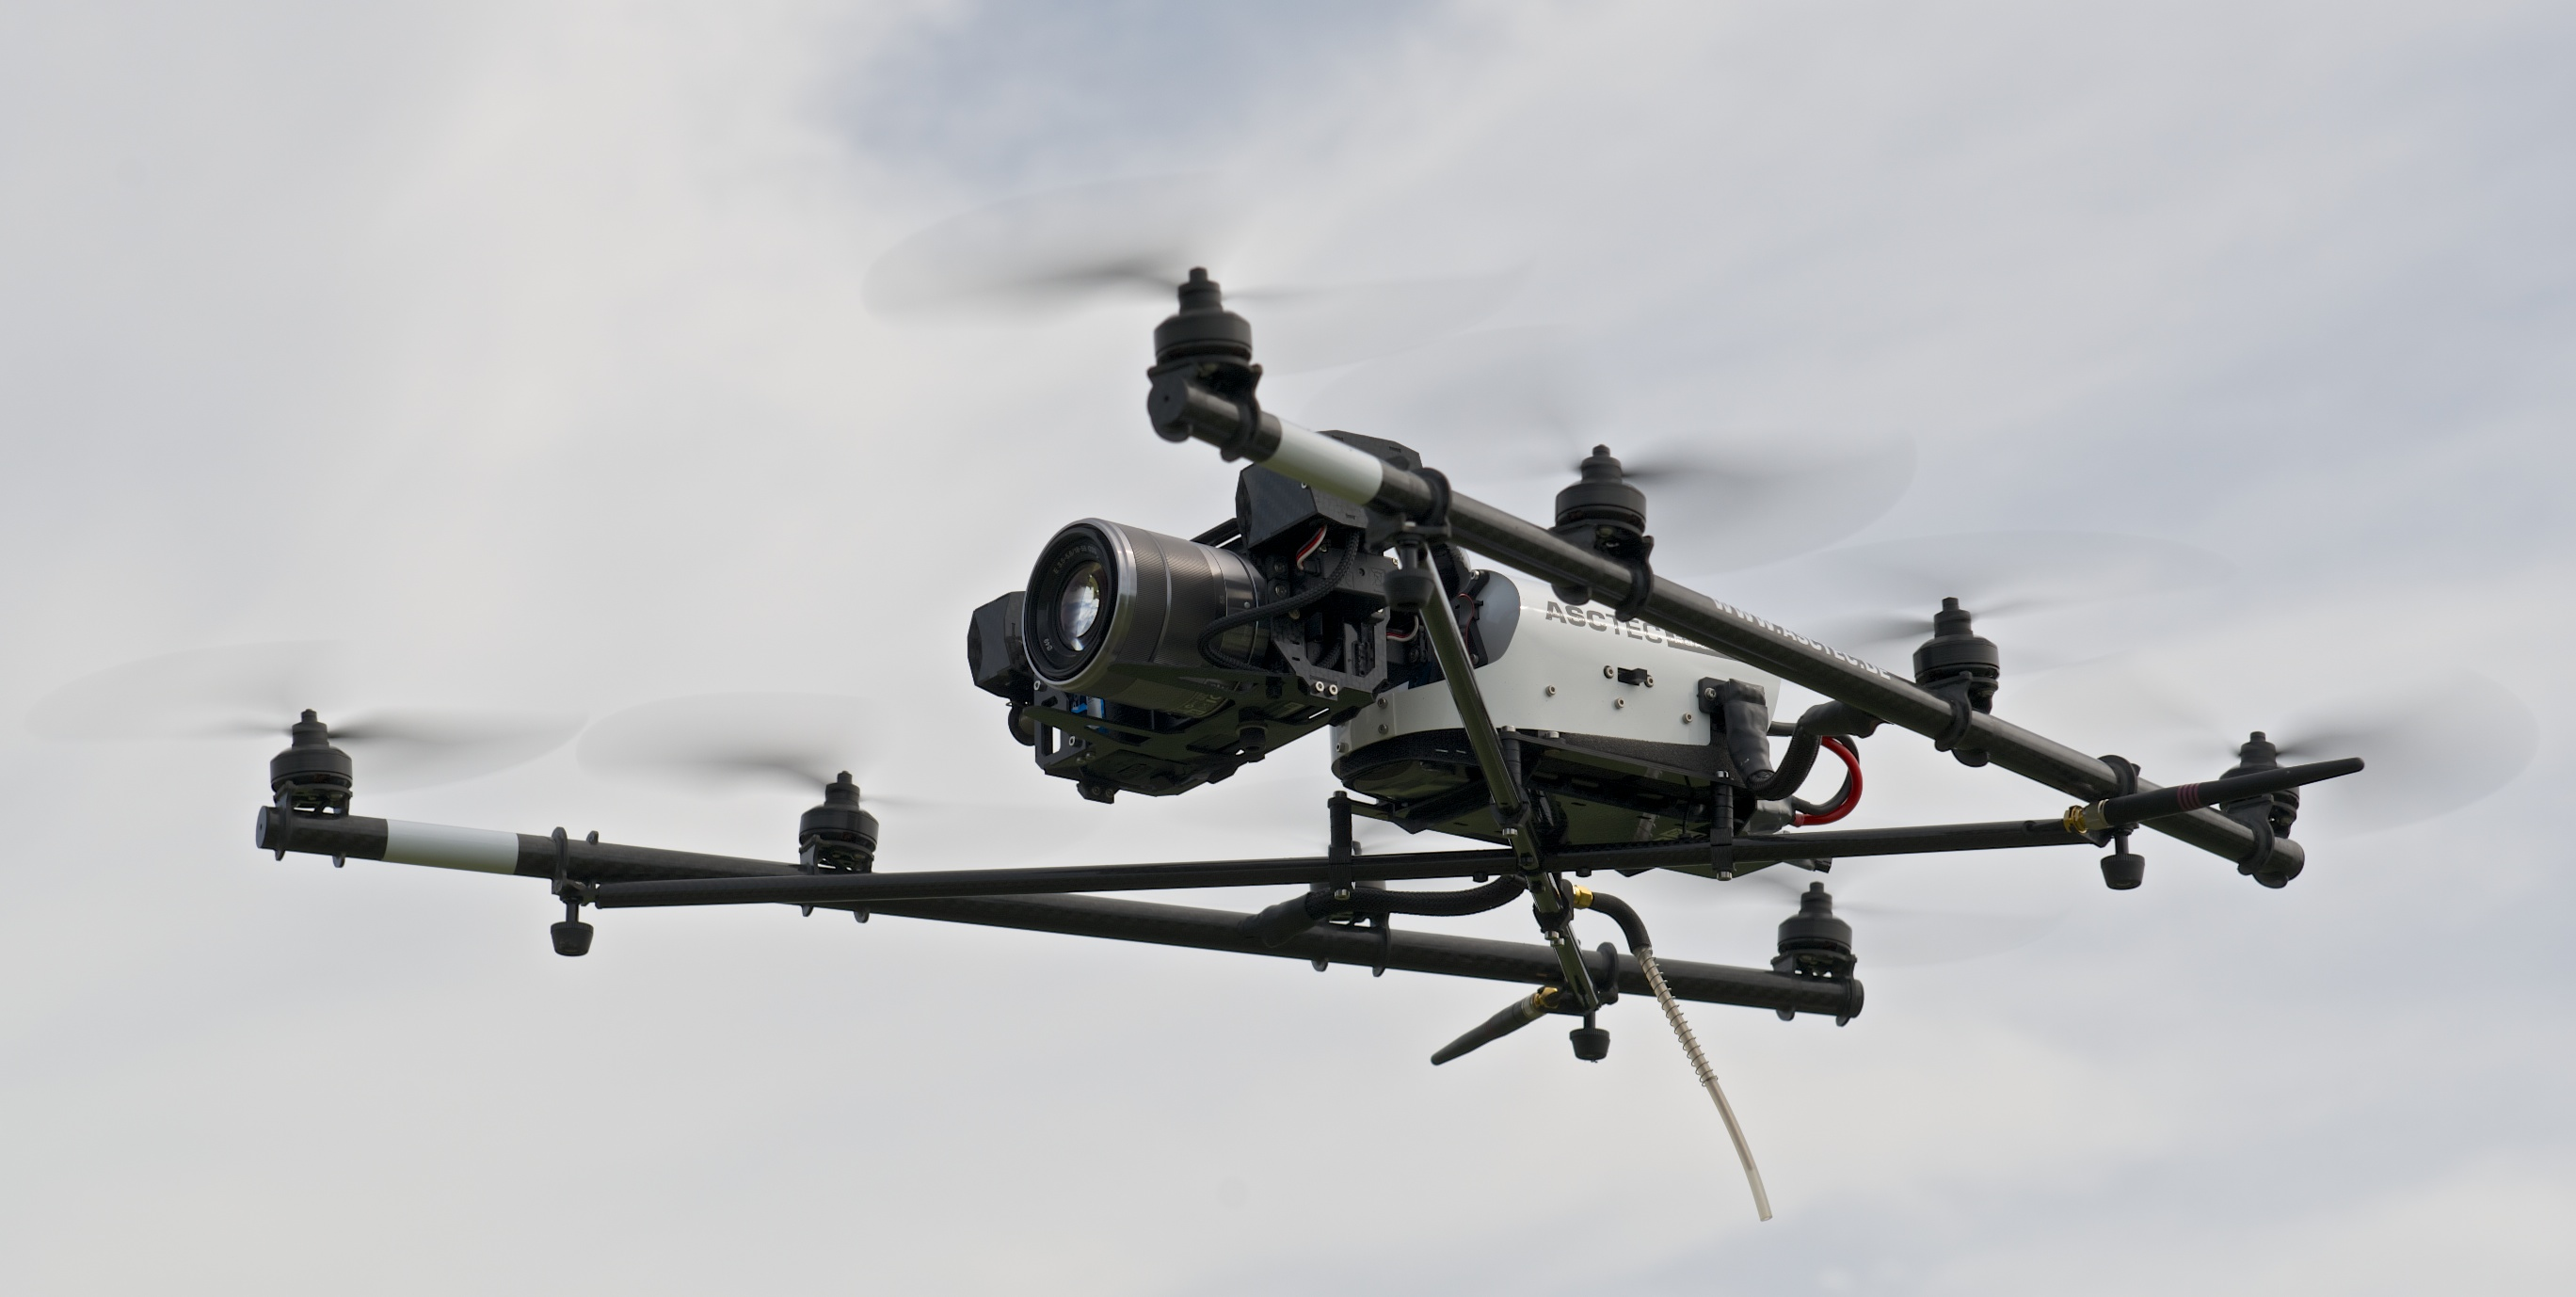
\includegraphics[width=0.9\linewidth]{uav.jpg}
        \caption{AscTec Falcon 8 octocopter}
    \end{subfigure}%\hskip2em
    \begin{subfigure}{.49\textwidth}
	\centering
        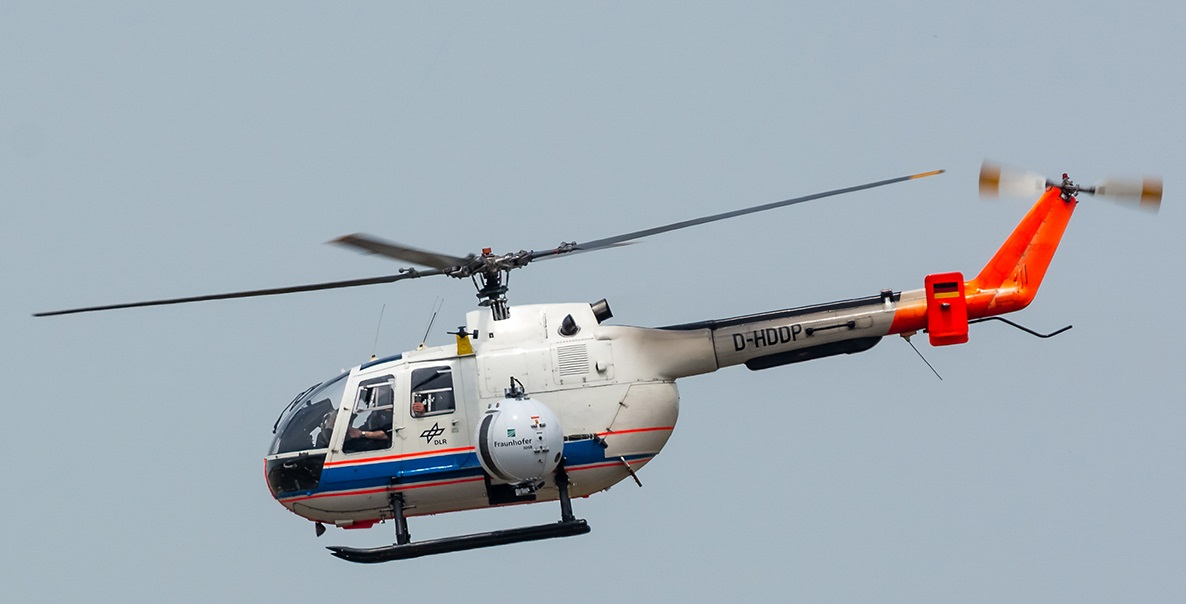
\includegraphics[width=0.9\linewidth]{aerial.jpg}
        \caption{DLR’s BO 105 research helicopter.}
    \end{subfigure}
\caption{Typical UAV and airborne platforms used in this paper}
\label{fig:platforms}
\end{figure}

\section{Characteristics}

Recent years have witnessed the fast development of UAVs. As a novel data acquisition platform, UAV bridges the gap between traditional airborne photogrammetry and terrestrial photogrammetry and demonstrates various advantages. Table \ref{tab:comp_charact} compares the main properties of UAV and traditional airborne platforms. With lower flight altitude, UAV imagery presents higher spatial resolution (approximately 1 cm/pixel) in contrast with imagery collected by traditional manned aircrafts (on the order of 25 cm/pixel), offering richer details of the scenes. Besides, conventional aerial photography platforms usually require big landing fields and pilots, and the flight plan is limited by air traffic and the weather. By contrast, UAVs only need small landing sites and can be remotely controlled, therefore they can work in severe weather conditions and even in hazardous areas with lower cost. In long term, UAVs offer superior temporal resolution as UAV-based survey tasks can be frequently updated according to users' demands, which is unpractical for manned aircrafts.
\begin{table}[H]
  \begin{center}
  %\footnotesize 
  \small
  \begin{tabular}{@{}p{.32\linewidth}p{.31\linewidth}p{.31\linewidth}@{}}
    \toprule
    {} & {\textbf{UAV platforms}} & {\textbf{Airborne platforms}} \\
    \cmidrule(){1-3}
    % %
    Spatial resolution/GSD& $cm$ & $dm$ \\
    \midrule
    Flexibility & Total & Flight plan needed\\&&weather dependent\\
    \midrule
    Update frequency & Ad-hoc & No or low\\
    \midrule
    % %
    System cost & $10 \sim1000$ k\euro{} & $1000\sim 10\,000$ k\euro{}\\ 
    \midrule
    Coverage & $\le 1 km^{2}$ & $10 \sim 10\,000km^{2}$ \\
    \midrule
    % %
    onborad GNSS/IMU accuracy & $m$ &$cm$\\
    \bottomrule
  \end{tabular}
  \end{center}
  \caption {Characteristics of UAV and traditional airborne platforms \cite{everaerts2008unmanned}}
\label{tab:comp_charact}
\end{table}


\begin{figure}[ht]\centering
 \begin{subfigure}{0.99\columnwidth}
\begin{tikzpicture}[
    zoomboxarray
]
    \node [image node] {\includegraphics[width=0.5\textwidth]{EK7P0089}};
    \zoombox[magnification=7,color code=yellow]{0.68,0.43}
    \zoombox[magnification=7,color code=red]{0.79,0.44}
    \zoombox[magnification=12,color code=blue]{0.63,0.62}
    \zoombox[magnification=12,color code=green]{0.62,0.7}
\end{tikzpicture} 
 \end{subfigure}

 \begin{subfigure}{0.244\columnwidth}
   \centering
\begin{tikzpicture}
   \centering
    \node[inner sep=0pt] (ima) at (0,0) {\includegraphics[cfbox=yellow,width=1\columnwidth]{G0000786}};    
 \end{tikzpicture}
 \end{subfigure}
  \begin{subfigure}{0.244\columnwidth}
   \centering
\begin{tikzpicture}
   \centering
    \node[inner sep=0pt] (ima) at (0,0) {\includegraphics[cfbox=red,width=1\columnwidth]{G0000852}};    
 \end{tikzpicture}
 \end{subfigure}
  \begin{subfigure}{0.244\columnwidth}
   \centering
\begin{tikzpicture}
   \centering
    \node[inner sep=0pt] (ima) at (0,0) {\includegraphics[cfbox=blue,angle=180,width=1\columnwidth]{IMG_1312}};    
 \end{tikzpicture}
 \end{subfigure}
  \begin{subfigure}{0.244\columnwidth}
   \centering
\begin{tikzpicture}
   \centering
    \node[inner sep=0pt] (ima) at (0,0) {\includegraphics[cfbox=green,width=1\columnwidth]{P1110932}};    
 \end{tikzpicture}
 \end{subfigure}
\vspace{1.1\baselineskip}
\centerline{\textbf{(c)}}
 \caption{Comparison of UAV and aerial imagery. (a) aerial image, (b) magnified areas in aerial image, (c) UAV images featuring corresponding areas}
\end{figure}
 
On the other hand, the coverage of UAV imagery is of limited extent, therefore UAVs are typically used for small-scale mapping as an efficient alternative to full-scale aerial mapping. The total costs of UAV platforms are thus expected to be kept to a minimum, which is usually at the cost of the accuracy of onboard GNSS/IMU systems. Table \ref{tab:comp_acc} compares the accuracy and price of onboard GNSS/IMU systems for UAV and conventional airborne platforms

\begin{table}[H]
  \begin{center}
  %\footnotesize 
  \small
  \begin{tabular}{@{}p{.23\linewidth}p{.25\linewidth}p{.4\linewidth}@{}}
    \toprule
    {} & {\textbf{GNSS/IMU on UAV (NEO-M8)}} & {\textbf{GNSS/IMU on manned aircraft (xOEM)}} \\
    \cmidrule(){1-3}
    % %
    Horizontal accuracy & $2.5$ m & $0.02$ m \\
    \midrule
    Vertical accuracy & $5$ m & $0.03$ m \\
    \midrule
Heading accuracy& $0.3^{\circ}$  & $0.05^{\circ}\sim0.1^{\circ}$\\
    \midrule
    % %
    Price & $30$ \euro{} & $15000$ \euro{}\\ 
    \bottomrule
  \end{tabular}
  \end{center}
  \caption {Comparison of onboard GNSS/IMU systems for UAVs and conventional manned aircrafts}
\label{tab:comp_acc}
\end{table}

Drones are increasingly being used for surveying building construction, road maintenance, and infrastructure inspections. Agricultural applications include crop inspection, and tracking farm animals. 




\chapter{State of the Art}
\label{chap:sota}
other cases for multi-modal data fusion?\\

other UAV geo-registration methods\\

other works about UAV image segmentation \\



%Example citations~\cite{barham2003xen, LIS}.



\chapter{Content}
\label{chap:content}

%\lipsum[1]

\section{Example Section}

%\lipsum[1-2]
%\lipsum[66]



\subsection{Example Table}

%\lipsum[1]

\begin{table}[thb]
    \renewcommand{\arraystretch}{1.3}
    \captionabove{Example Table.}
    \label{table:example_table}
    \centering

    \begin{tabular}{|r|l|}
      \hline
      7C0         & hexadecimal \\
      3700        & octal \\
      \cline{2-2}
      11111000000 & binary \\
      \hline
      \hline
      1984        & decimal \\
      \hline
    \end{tabular}
\end{table}


\lipsum[2-4]



\subsection{Example Plot}

\lipsum[1]

\begin{figure}[thb]
    \centering

    \begin{tikzpicture}
        \begin{loglogaxis}[
            xlabel={Degrees of freedom},
            ylabel={$L_2$ Error}
            ]
            \addplot coordinates {
              (5,8.312e-02)    (17,2.547e-02)   (49,7.407e-03)
              (129,2.102e-03)  (321,5.874e-04)  (769,1.623e-04)
              (1793,4.442e-05) (4097,1.207e-05) (9217,3.261e-06)
            };

            \addplot coordinates{
              (7,8.472e-02)    (31,3.044e-02)    (111,1.022e-02)
              (351,3.303e-03)  (1023,1.039e-03)  (2815,3.196e-04)
              (7423,9.658e-05) (18943,2.873e-05) (47103,8.437e-06)
            };

            \addplot coordinates{
              (9,7.881e-02)     (49,3.243e-02)    (209,1.232e-02)
              (769,4.454e-03)   (2561,1.551e-03)  (7937,5.236e-04)
              (23297,1.723e-04) (65537,5.545e-05) (178177,1.751e-05)
            };

            \addplot coordinates{
              (11,6.887e-02)    (71,3.177e-02)     (351,1.341e-02)
              (1471,5.334e-03)  (5503,2.027e-03)   (18943,7.415e-04)
              (61183,2.628e-04) (187903,9.063e-05) (553983,3.053e-05)
            };

            \addplot coordinates{
              (13,5.755e-02)     (97,2.925e-02)     (545,1.351e-02)
              (2561,5.842e-03)   (10625,2.397e-03)  (40193,9.414e-04)
              (141569,3.564e-04) (471041,1.308e-04) (1496065,4.670e-05)
            };

            \addplot coordinates{
              (15,6.75e-02)     (123,3.425e-02)     (745,1.751e-02)
              (5561,5.942e-03)   (30625,2.197e-03)  (90193,9.714e-04)
              (341569,3.564e-04) (871041,1.708e-04) (1896065,8.670e-05)
            };
            \legend{$d=2$,$d=3$,$d=4$,$d=5$,$d=6$,$d=7$}
        \end{loglogaxis}
    \end{tikzpicture}

    \caption{Example Plot.}

    \label{fig:example_plot}
\end{figure}

\lipsum[3]
\lipsum[66]



\subsection{Example Barchart}

\lipsum[1]

\begin{figure}[thb]
    \centering

    \begin{tikzpicture}
        \begin{axis}[
            ybar               = 5pt, % configures `bar shift'
            xmajorgrids        = false,
            x tick label style = {
              /pgf/number format/1000 sep =},
            xtick              = {1930, 1940, 1950},
            ylabel             = y-Axis,
            enlarge x limits   = 0.25,
            ymin               = 2e7,
            ymax               = 8e7,
            bar width          = 9pt,
            point meta         = y *10^-7, % the displayed number
            nodes near coords,
            ]
            \addplot
            coordinates {(1930,70e6) (1940,33e6)
              (1950,40e6)};

            \addplot
            coordinates {(1930,65e6) (1940,42e6)
              (1950,43e6)};

            \addplot
            coordinates {(1930,45e6) (1940,47e6)
              (1950,34e6)};

            \addplot
            coordinates {(1930,34e6) (1940,37e6)
              (1950,38e6)};

            \addplot
            coordinates {(1930,28e6) (1940,27e6)
              (1950,30e6)};

            \addplot
            coordinates {(1930,24e6) (1940,31e6)
              (1950,33e6)};

            \legend{One, Two, Three, Four, Five, Six}
        \end{axis}
    \end{tikzpicture}

    \caption{Example Barchart.}

    \label{fig:example_barchart}
\end{figure}

\lipsum[3]
\lipsum[66]



\subsection{Example Source Code}

\lipsum[1]

\begin{lstlisting}[
    language = C,
    caption  = {Example Source Code},
    label    = {list:example_src}
]
#include <stdio.h>

void quick_sort (int *a, int n) {
    int i, j, p, t;
    if (n < 2)
        return;
    p = a[n / 2];
    for (i = 0, j = n - 1;; i++, j--) {
        while (a[i] < p)
            i++;
        while (p < a[j])
            j--;
        if (i >= j)
            break;
        t = a[i];
        a[i] = a[j];
        a[j] = t;
    }
    quick_sort(a, i);
    quick_sort(a + i, n - i);
}

/* main routine */
int main (void) {
    int a[] = {4, 65, 2, -31, 0, 99, 2, 83, 782, 1};
    int n = sizeof a / sizeof a[0];
    int i;
    for (i = 0; i < n; i++)
        printf("%d%s", a[i], i == n - 1 ? "\n" : " ");
    quick_sort(a, n);
    for (i = 0; i < n; i++)
        printf("%d%s", a[i], i == n - 1 ? "\n" : " ");
    return 0;
}
\end{lstlisting}



\subsection{Example Subsection}

\lipsum[1]



\subsubsection{Example SubSubSection}

\lipsum[9]



\subsubsection{Example SubSubSection}

\lipsum[10]



\chapter{Conclusion \& Outlook}
\label{chap:conclusion}

\lipsum[1-4]



%-------------------------------------------------------------------------------
% Bibliography
%-------------------------------------------------------------------------------
%\backmatter
\bibliographystyle{unsrturl-custom}
\bibliography{bibliography}



%-------------------------------------------------------------------------------
% Appendix
%-------------------------------------------------------------------------------
\appendix
\chapter{Additional Stuff}

\lipsum[1-4]

\end{document}
